\documentclass{beamer}
\usetheme[style=plain]{uu}
\usefonttheme{professionalfonts}

\usepackage{fontspec}

%% Standard packages
\usepackage{unicode-math}
\usepackage{mathtools}
\usepackage{amsmath}
\usepackage{graphicx}
\usepackage{hyperref}
\usepackage{color}
\usepackage{url}
\usepackage{acronym}
\usepackage{cite}
\usepackage{listings}
\usepackage{graphicx}
\usepackage{epstopdf}
\usepackage{pgfplotstable}
\usepackage{booktabs}
\usepackage{colortbl}
\usepackage{lmodern}
%\usepackage[norndcorners,customcolors]{hf-tikz}

%% Code
% \usepackage{minted}
% \usepackage{fancyvrb}
% \usemintedstyle{default}


%% Agda
\usepackage{catchfilebetweentags}
\usepackage{src/agda/latex/agda}
\newcommand{\AK}{\AgdaKeyword}
\newcommand{\AS}{\AgdaString}
\newcommand{\AY}{\AgdaSymbol}
\newcommand{\AN}{\AgdaNumber}
\newcommand{\AB}{\AgdaBound}
\newcommand{\AO}{\AgdaOperator}
\newcommand{\AI}{\AgdaInductiveConstructor}
\newcommand{\AC}{\AgdaCoinductiveConstructor}
\newcommand{\AD}{\AgdaDatatype}
\newcommand{\AF}{\AgdaFunction}
\newcommand{\AM}{\AgdaModule}
\newcommand{\AL}{\AgdaField}
\newcommand{\AR}{\AgdaArgument}
\newcommand{\AT}{\AgdaIndent}
\newcommand{\ARR}{\AgdaRecord}

\lstset{escapechar=§}


%% PDF metainformation
\usepackage{datetime}
\usepackage{ifpdf}
\ifpdf
\pdfinfo{
    /Author (Philipp Hausmann)
    /Title (Agda UHC Backend Prototype: On the way to a decent Agda compiler.)
    /Keywords (Agda, Dependently-typed programming, Functional programming, Compilers, Dependent types, Coq, Lava, Coquet)
    /CreationDate (D:\pdfdate)
}
\fi


%% LaTeX meta-information
\title[Agda UHC Backend]{Agda Backends: A survey and a UHC backend prototype}
\date{\today}

%% Author after \begin{document}

\institute[Utrecht University] {
    Department of Information and Computing Sciences \\
    Utrecht University
}

%\subject{DSL, EDSL, Agda, Dependently-typed programming, Functional programming, Hardware Description, Dependent types, Coq, Lava, Coquet}



\defbeamertemplate{section page}{mine}[1][]{%
    \begin{centering}
        {\usebeamerfont{section name}\usebeamercolor[fg]{section name}#1}
        \vskip1em\par
        \begin{beamercolorbox}[sep=12pt,center]{part title}
            \usebeamerfont{section title}\insertsection\par
        \end{beamercolorbox}
    \end{centering}
}

\defbeamertemplate{subsection page}{mine}[1][]{%
    \begin{centering}
        {\usebeamerfont{subsection name}\usebeamercolor[fg]{subsection name}#1}
        \vskip1em\par
        \begin{beamercolorbox}[sep=8pt,center,#1]{part title}
            \usebeamerfont{subsection title}\insertsubsection\par
        \end{beamercolorbox}
    \end{centering}
}


%% The document itself
\AtBeginSubsection{\frame{\subsectionpage}}
\begin{document}
    \author[P. Hausmann]{
        \begin{tabular}{r@{ }l}
            Author:     & Philipp Hausmann \\
                        & \small{\texttt{<p.hausmann@students.uu.nl>}} \\[2ex]
            Supervisors: & Wouter Swierstra \\
                        & \small{\texttt{<w.s.swierstra@uu.nl>}} \\
                        & Atze Dijkstra \\
                        & \small{\texttt{<atze@uu.nl>}}
        \end{tabular}
    }

    \setbeamertemplate{section page}[mine][]
    \setbeamertemplate{subsection page}[mine][]

    \begin{frame}
        \titlepage
    \end{frame}

    \begin{frame}
        \frametitle{Table of Contents}
        \tableofcontents
    \end{frame}

    % Agda introduction
    % overview existing backends
    % UHC backend
    %   comparison uhc core / epic
    %   challenges?
    %   uhc changes
    %   demonstration
    % Future work
    %   Master thesis / stdlib, ffi
    %   merge with agda
    %   
    % Other future work
    %   cabal support for Agda/UHC


    %% Sections
    \section{Agda Introduction}
\begin{frame}[fragile]{Agda Introduction}
\begin{itemize}
\item Why dependent types?
\pause \item
\begin{lstlisting}[language=Haskell]
head :: forall a . List a -> a
head (x:xs) = x
head [] = error "something went wrong..."
\end{lstlisting}
\pause \item Runtime crashes are possible in Haskell!
\end{itemize}
\end{frame}

\begin{frame}[fragile]{Agda Introduction}
\begin{itemize}
\item How to make sure at compile time that this doesn't happen?
\item We need to encode the length of lists in the type
\end{itemize}
\pause
\begin{code}%
\>\AgdaKeyword{data} \AgdaDatatype{Nat} \AgdaSymbol{:} \AgdaPrimitiveType{Set} \AgdaKeyword{where}\<%
\\
\>[0]\AgdaIndent{2}{}\<[2]%
\>[2]\AgdaInductiveConstructor{zero} \AgdaSymbol{:} \AgdaDatatype{Nat}\<%
\\
\>[0]\AgdaIndent{2}{}\<[2]%
\>[2]\AgdaInductiveConstructor{succ} \AgdaSymbol{:} \AgdaDatatype{Nat} \AgdaSymbol{→} \AgdaDatatype{Nat}\<%
\end{code}
\pause
\vspace{0.5cm}
\begin{code}%
\>\AgdaKeyword{data} \AgdaDatatype{Vec} \AgdaSymbol{:} \AgdaSymbol{(}\AgdaBound{A} \AgdaSymbol{:} \AgdaPrimitiveType{Set}\AgdaSymbol{)} \AgdaSymbol{→} \AgdaSymbol{(}\AgdaBound{n} \AgdaSymbol{:} \AgdaDatatype{Nat}\AgdaSymbol{)} \AgdaSymbol{→} \AgdaPrimitiveType{Set} \AgdaKeyword{where}\<%
\\
\>[0]\AgdaIndent{2}{}\<[2]%
\>[2]\AgdaInductiveConstructor{nil} \<[7]%
\>[7]\AgdaSymbol{:} \AgdaSymbol{∀} \AgdaSymbol{\{}\AgdaBound{A}\AgdaSymbol{\}} \AgdaSymbol{→} \AgdaDatatype{Vec} \AgdaBound{A} \AgdaInductiveConstructor{zero}\<%
\\
\>[0]\AgdaIndent{2}{}\<[2]%
\>[2]\AgdaInductiveConstructor{cons} \AgdaSymbol{:} \AgdaSymbol{∀} \AgdaSymbol{\{}\AgdaBound{A} \AgdaBound{n}\AgdaSymbol{\}} \AgdaSymbol{→} \AgdaBound{A} \AgdaSymbol{→} \AgdaDatatype{Vec} \AgdaBound{A} \AgdaBound{n} \AgdaSymbol{→} \AgdaDatatype{Vec} \AgdaBound{A} \AgdaSymbol{(}\AgdaInductiveConstructor{succ} \AgdaBound{n}\AgdaSymbol{)}\<%
\end{code}
\end{frame}

\begin{frame}[fragile]{Cont.}
We can now write the head function in Agda
\begin{code}%
\>\AgdaFunction{head1} \AgdaSymbol{:} \AgdaSymbol{∀} \AgdaSymbol{\{}\AgdaBound{A} \AgdaBound{n}\AgdaSymbol{\}} \AgdaSymbol{→} \AgdaDatatype{Vec} \AgdaBound{A} \AgdaBound{n} \AgdaSymbol{→} \AgdaBound{A}\<%
\\
\>\AgdaFunction{head1} \AgdaSymbol{(}\AgdaInductiveConstructor{cons} \AgdaBound{x} \AgdaBound{xs}\AgdaSymbol{)} \AgdaSymbol{=} \AgdaBound{x}\<%
\\
\>\AgdaFunction{head1} \AgdaInductiveConstructor{nil} \AgdaSymbol{=} \AgdaBound{????}\<%
\end{code}
\pause
This will not type check!
\par
\pause
\vspace{0.5cm}
\begin{code}%
\>\AgdaFunction{head2} \AgdaSymbol{:} \AgdaSymbol{∀} \AgdaSymbol{\{}\AgdaBound{A} \AgdaBound{n}\AgdaSymbol{\}} \AgdaSymbol{→} \AgdaDatatype{Vec} \AgdaBound{A} \AgdaSymbol{(}\AgdaInductiveConstructor{succ} \AgdaBound{n}\AgdaSymbol{)} \AgdaSymbol{→} \AgdaBound{A}\<%
\\
\>\AgdaFunction{head2} \AgdaSymbol{(}\AgdaInductiveConstructor{cons} \AgdaBound{x} \AgdaBound{xs}\AgdaSymbol{)} \AgdaSymbol{=} \AgdaBound{x}\<%
\end{code}
The typechecker now knows that the nil-case cannot happen!
\end{frame}

\begin{frame}{Agda Summary}
\begin{itemize}
\item Values can be used as types
\item Types cannot influence value of an expression
\item Functions need to be total
\end{itemize}
\end{frame}

    \section{Existing Backends}

\begin{frame}[fragile]{Agda Architecture}
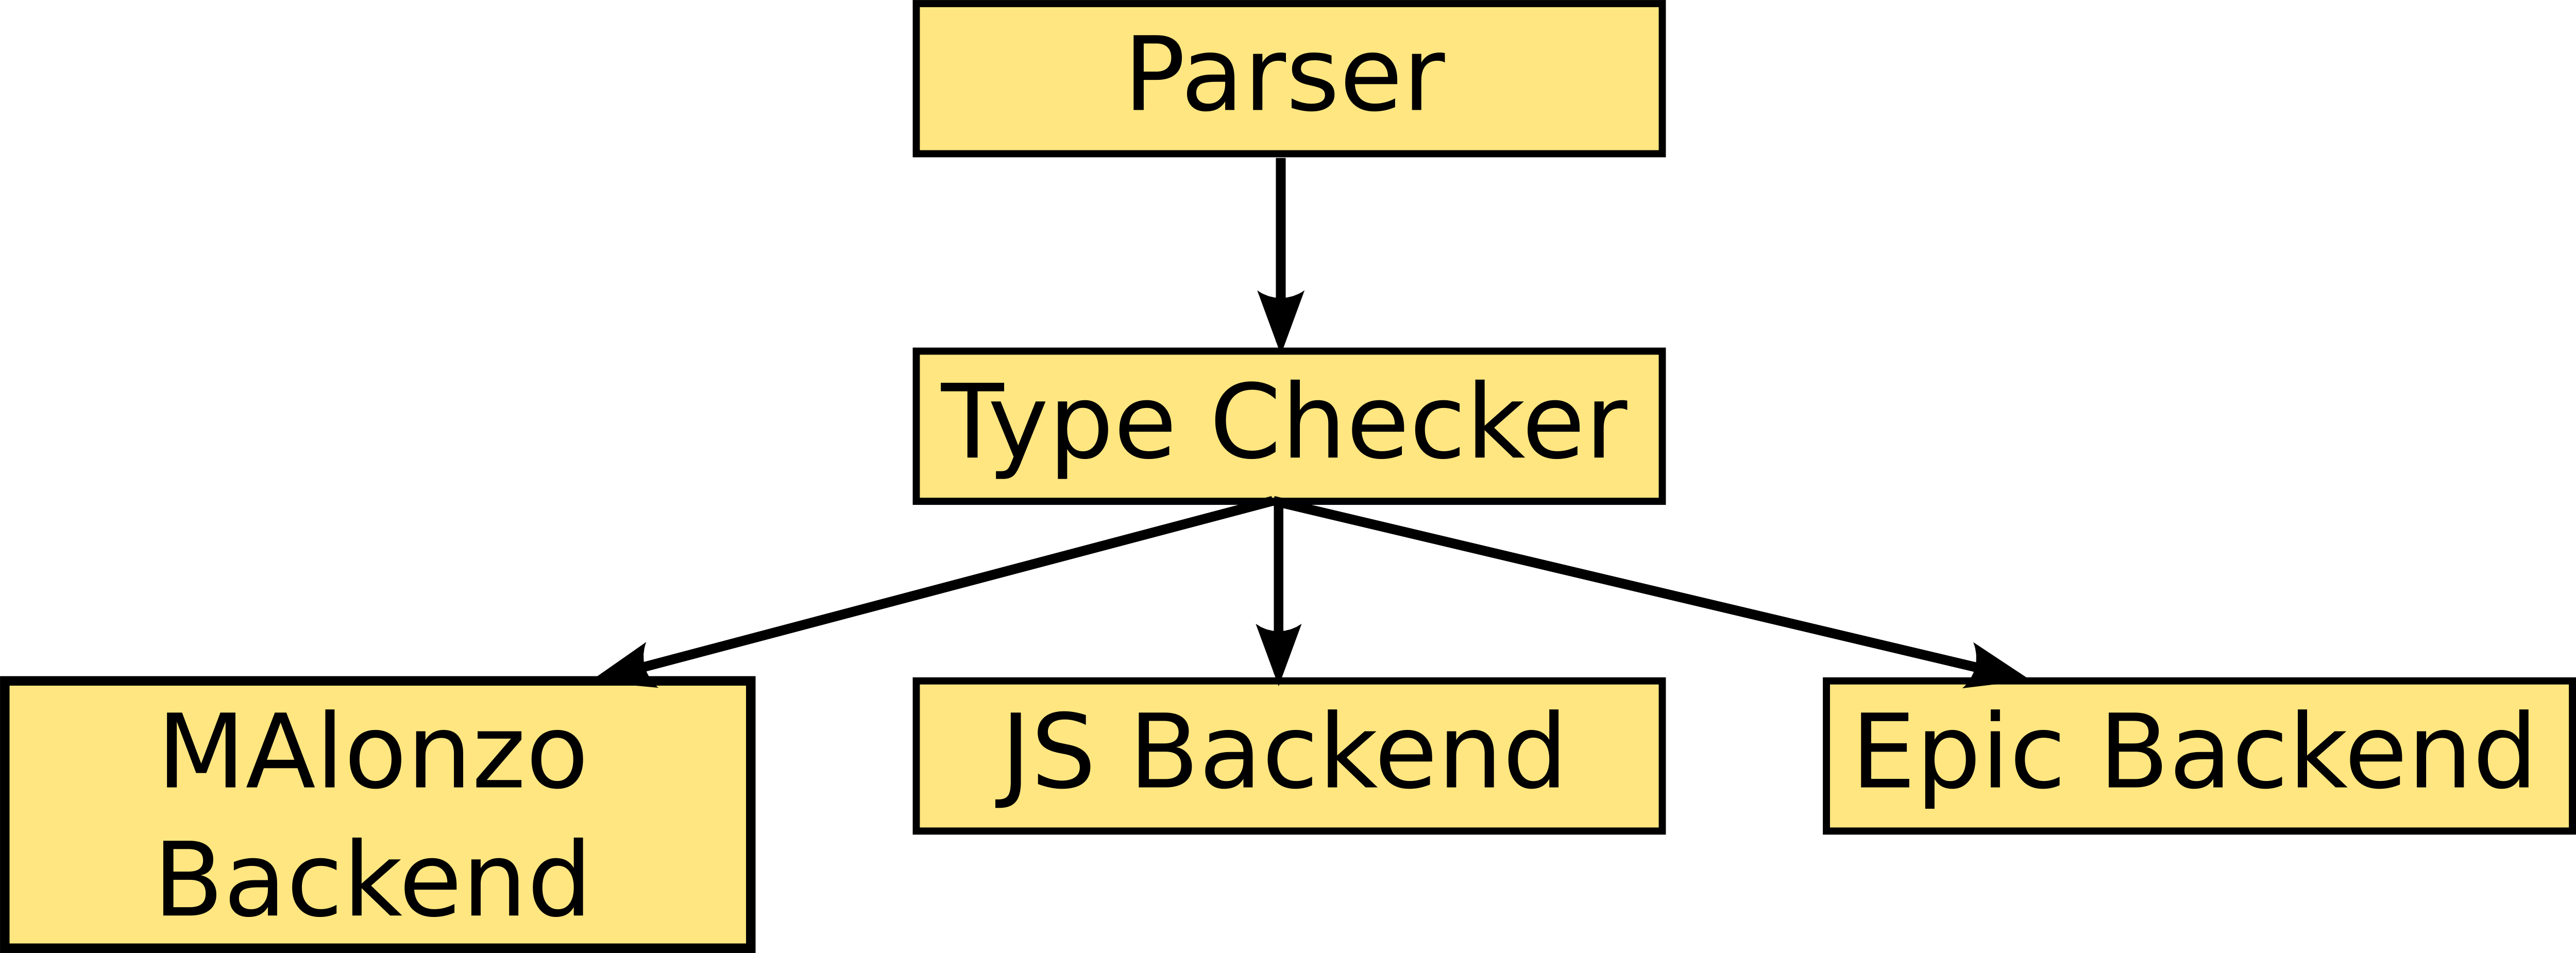
\includegraphics[width=250px]{agda-arch.png}
\end{frame}

\subsection{MAlonzo backend}
\begin{frame}{MAlonzo backend}
\begin{itemize}
\item Targets Haskell
\item Maintained
\item Relies on GHC for optimizations
\end{itemize}
\end{frame}


\begin{frame}{MAlonzo - FFI}
\begin{itemize}
\item Provides simple FFI to haskell
\item Very limited
  \begin{itemize}
    \item No class support
    \item Can't export Agda datatypes
    \item Not automatic
  \end{itemize}
\end{itemize}
\end{frame}

\begin{frame}[fragile]{MAlonzo - FFI}
\begin{code}%
\>\AgdaSymbol{\{-\#} \AgdaKeyword{IMPORT} Data.List \AgdaSymbol{\#-\}}\<%
\\
%
\\
\>\AgdaKeyword{data} \AgdaDatatype{List} \AgdaSymbol{:} \AgdaSymbol{(}\AgdaBound{A} \AgdaSymbol{:} \AgdaPrimitiveType{Set}\AgdaSymbol{)} \AgdaSymbol{->} \AgdaPrimitiveType{Set} \AgdaKeyword{where}\<%
\\
\>[0]\AgdaIndent{2}{}\<[2]%
\>[2]\AgdaInductiveConstructor{nil} \AgdaSymbol{:} \AgdaSymbol{∀} \AgdaSymbol{\{}\AgdaBound{A}\AgdaSymbol{\}} \AgdaSymbol{→} \AgdaDatatype{List} \AgdaBound{A}\<%
\\
\>[0]\AgdaIndent{2}{}\<[2]%
\>[2]\AgdaInductiveConstructor{cons} \AgdaSymbol{:} \AgdaSymbol{∀} \AgdaSymbol{\{}\AgdaBound{A}\AgdaSymbol{\}} \AgdaSymbol{→} \AgdaBound{A} \AgdaSymbol{→} \AgdaDatatype{List} \AgdaBound{A} \AgdaSymbol{→} \AgdaDatatype{List} \AgdaBound{A}\<%
\\
\>\AgdaSymbol{\{-\#} \AgdaKeyword{COMPILED\_DATA} \AgdaDatatype{List} Data.List nil cons \AgdaSymbol{\#-\}}\<%
\\
%
\\
\>\AgdaKeyword{postulate}\<%
\\
\>[0]\AgdaIndent{2}{}\<[2]%
\>[2]\AgdaPostulate{head} \AgdaSymbol{:} \AgdaSymbol{∀} \AgdaSymbol{\{}\AgdaBound{A}\AgdaSymbol{\}} \AgdaSymbol{→} \AgdaDatatype{List} \AgdaBound{A} \AgdaSymbol{->} \AgdaBound{A}\<%
\\
\>\AgdaSymbol{\{-\#} \AgdaKeyword{COMPILED} \AgdaPostulate{head} Data.List.head \AgdaSymbol{\#-\}}\<%
\\
\>\<%
\end{code}
\end{frame}

\begin{frame}[fragile]{MAlonzo - Code Generation}
\begin{code}%
\>\AgdaFunction{vecToStr} \AgdaSymbol{:} \AgdaSymbol{∀} \AgdaSymbol{\{}\AgdaBound{A} \AgdaBound{m}\AgdaSymbol{\}} \AgdaSymbol{→} \AgdaSymbol{(}\AgdaBound{A} \AgdaSymbol{→} \AgdaPostulate{String}\AgdaSymbol{)}\<%
\\
\>[2]\AgdaIndent{4}{}\<[4]%
\>[4]\AgdaSymbol{→} \AgdaDatatype{Vec} \AgdaBound{A} \AgdaBound{m} \AgdaSymbol{→} \AgdaPostulate{String}\<%
\\
\>\AgdaFunction{vecToStr} \AgdaBound{f} \AgdaInductiveConstructor{[]} \AgdaSymbol{=} \AgdaString{""}\<%
\\
\>\AgdaFunction{vecToStr} \AgdaBound{f} \AgdaSymbol{(}\AgdaBound{x} \AgdaInductiveConstructor{::} \AgdaBound{xs}\AgdaSymbol{)} \AgdaSymbol{=} \AgdaString{", "} \AgdaFunction{++} \AgdaSymbol{((}\AgdaBound{f} \AgdaBound{x}\AgdaSymbol{)}\<%
\\
\>[2]\AgdaIndent{4}{}\<[4]%
\>[4]\AgdaFunction{++} \AgdaSymbol{(}\AgdaFunction{vecToStr} \AgdaBound{f} \AgdaBound{xs}\AgdaSymbol{))}\<%
\end{code}

%\ExecuteMetaData[src/agda/latex/HelloDatHS.tex]{vecToStr}

%\input{src/agda/latex/HelloDat_HS.tex}
\end{frame}

\begin{frame}[fragile]{MAlonzo - Code Generation}
\begin{lstlisting}[language=Haskell,basicstyle=\scriptsize]
d55 v0 v1 v2 v3
  = MAlonzo.RTE.mazCoerce
      (d_1_55 (MAlonzo.RTE.mazCoerce v0)
         (MAlonzo.RTE.mazCoerce v1)
         (MAlonzo.RTE.mazCoerce v2)
         (MAlonzo.RTE.mazCoerce v3))
  where d_1_55 v0 v1 v2 (C51 v3 v4 v5)
          = MAlonzo.RTE.mazCoerce
              (d33 (MAlonzo.RTE.mazCoerce ", ")
                 (MAlonzo.RTE.mazCoerce
  (d33 (MAlonzo.RTE.mazCoerce (v2 (MAlonzo.RTE.mazCoerce v4)))
     (MAlonzo.RTE.mazCoerce
        (d55 (MAlonzo.RTE.mazCoerce v0) (MAlonzo.RTE.mazCoerce v3)
           (MAlonzo.RTE.mazCoerce v2)
           (MAlonzo.RTE.mazCoerce v5))))))
        d_1_55 v0 v1 v2 v3 = MAlonzo.RTE.mazIncompleteMatch name55
\end{lstlisting}
\end{frame}

\begin{frame}{MAlonzo - Summary}
\begin{itemize}
  \item Produces 'strange' haskell code
  \item Can lead to size blow-up
  \begin {itemize}
    \item 84 lines Agda - 250'000 lines Haskell - 300 Mb executable (CITE)
  \end{itemize}
\end{itemize}
\end{frame}

\subsection{JS backend}
\begin{frame}{JS backend}
\begin{itemize}
\item Targets Javascript
\item Not maintained
\item Very similar to MAlonzo
\end{itemize}
\end{frame}

\subsection{Epic backend}
\begin{frame}{Epic backend}
\begin{itemize}
\item Targets Epic
\item Not maintained
\end{itemize}
\end{frame}

\begin{frame}{Epic}
\begin{itemize}
\item Untyped-lambda calculus with some extensions
\item Intended as building block for compilers
\item Also not maintained
\end{itemize}
\end{frame}

\begin{frame}[fragile]{Epic Language}
\begin{tabular}{c r l}
\hline
\multicolumn{3}{l}{Epic Language} \\
\hline
$t$ & $::=$ & $x$            \\
& \textbar & $t$ $\vec{t}$            \\
& \textbar & $\lambda x \rightarrow t$  \\
& \textbar & Con $i$ $\vec{t}$         \\
& \textbar & if $t$ then $t$ else $t$  \\
& \textbar & case $t$ of $\vec{alt}$   \\
& \textbar & let $x$ = $t$ in $t$      \\
& &                                    \\
& \textbar & lazy $t$                  \\
& \textbar & $t$ $!$ $i$               \\
& \textbar & $i$                       \\
\\
$alt$ & ::= & Con $i$ $\vec{x}$ $\rightarrow$ $t$     \\
& \textbar & $i$ $\rightarrow$ $t$                    \\
& \textbar & default $\rightarrow$ $t$               
\end{tabular}
\end{frame}

\begin{frame}[fragile]{Epic - Nat Optimizations}
\begin{itemize}
\item \begin{code}%
\>\AgdaKeyword{data} \AgdaDatatype{Nat} \AgdaSymbol{:} \AgdaPrimitiveType{Set} \AgdaKeyword{where}\<%
\\
\>[0]\AgdaIndent{2}{}\<[2]%
\>[2]\AgdaInductiveConstructor{zero} \AgdaSymbol{:} \AgdaDatatype{Nat}\<%
\\
\>[0]\AgdaIndent{2}{}\<[2]%
\>[2]\AgdaInductiveConstructor{succ} \AgdaSymbol{:} \AgdaDatatype{Nat} \AgdaSymbol{->} \AgdaDatatype{Nat}\<%
\\
\>\AgdaSymbol{\{-\#} \AgdaKeyword{BUILTIN} NATURAL \AgdaDatatype{Nat} \AgdaSymbol{\#-\}}\<%
\\
\>\<%
\end{code}
\item Naive translation is horribly slow
\item Can be transformed into arbitrary precision Integers
\item Automatic detection of Nat-like datatypes
\end{itemize}
\end{frame}

\begin{frame}{Nat Performance}
TODO add graph comparing performance for MAlonzo and Epic
\end{frame}


\begin{frame}{Comparison}
\end{frame}

    \section{UHC Backend}

% two steps, first without mod
\begin{frame}[fragile]{UHC Compiler}
\hspace{3cm}
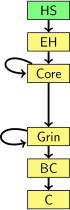
\includegraphics{uhc-arch-extr.png}
\footcite{dijkstra2009architecture}
\end{frame}

\begin{frame}[fragile]{UHC Compiler}
\hspace{3cm}
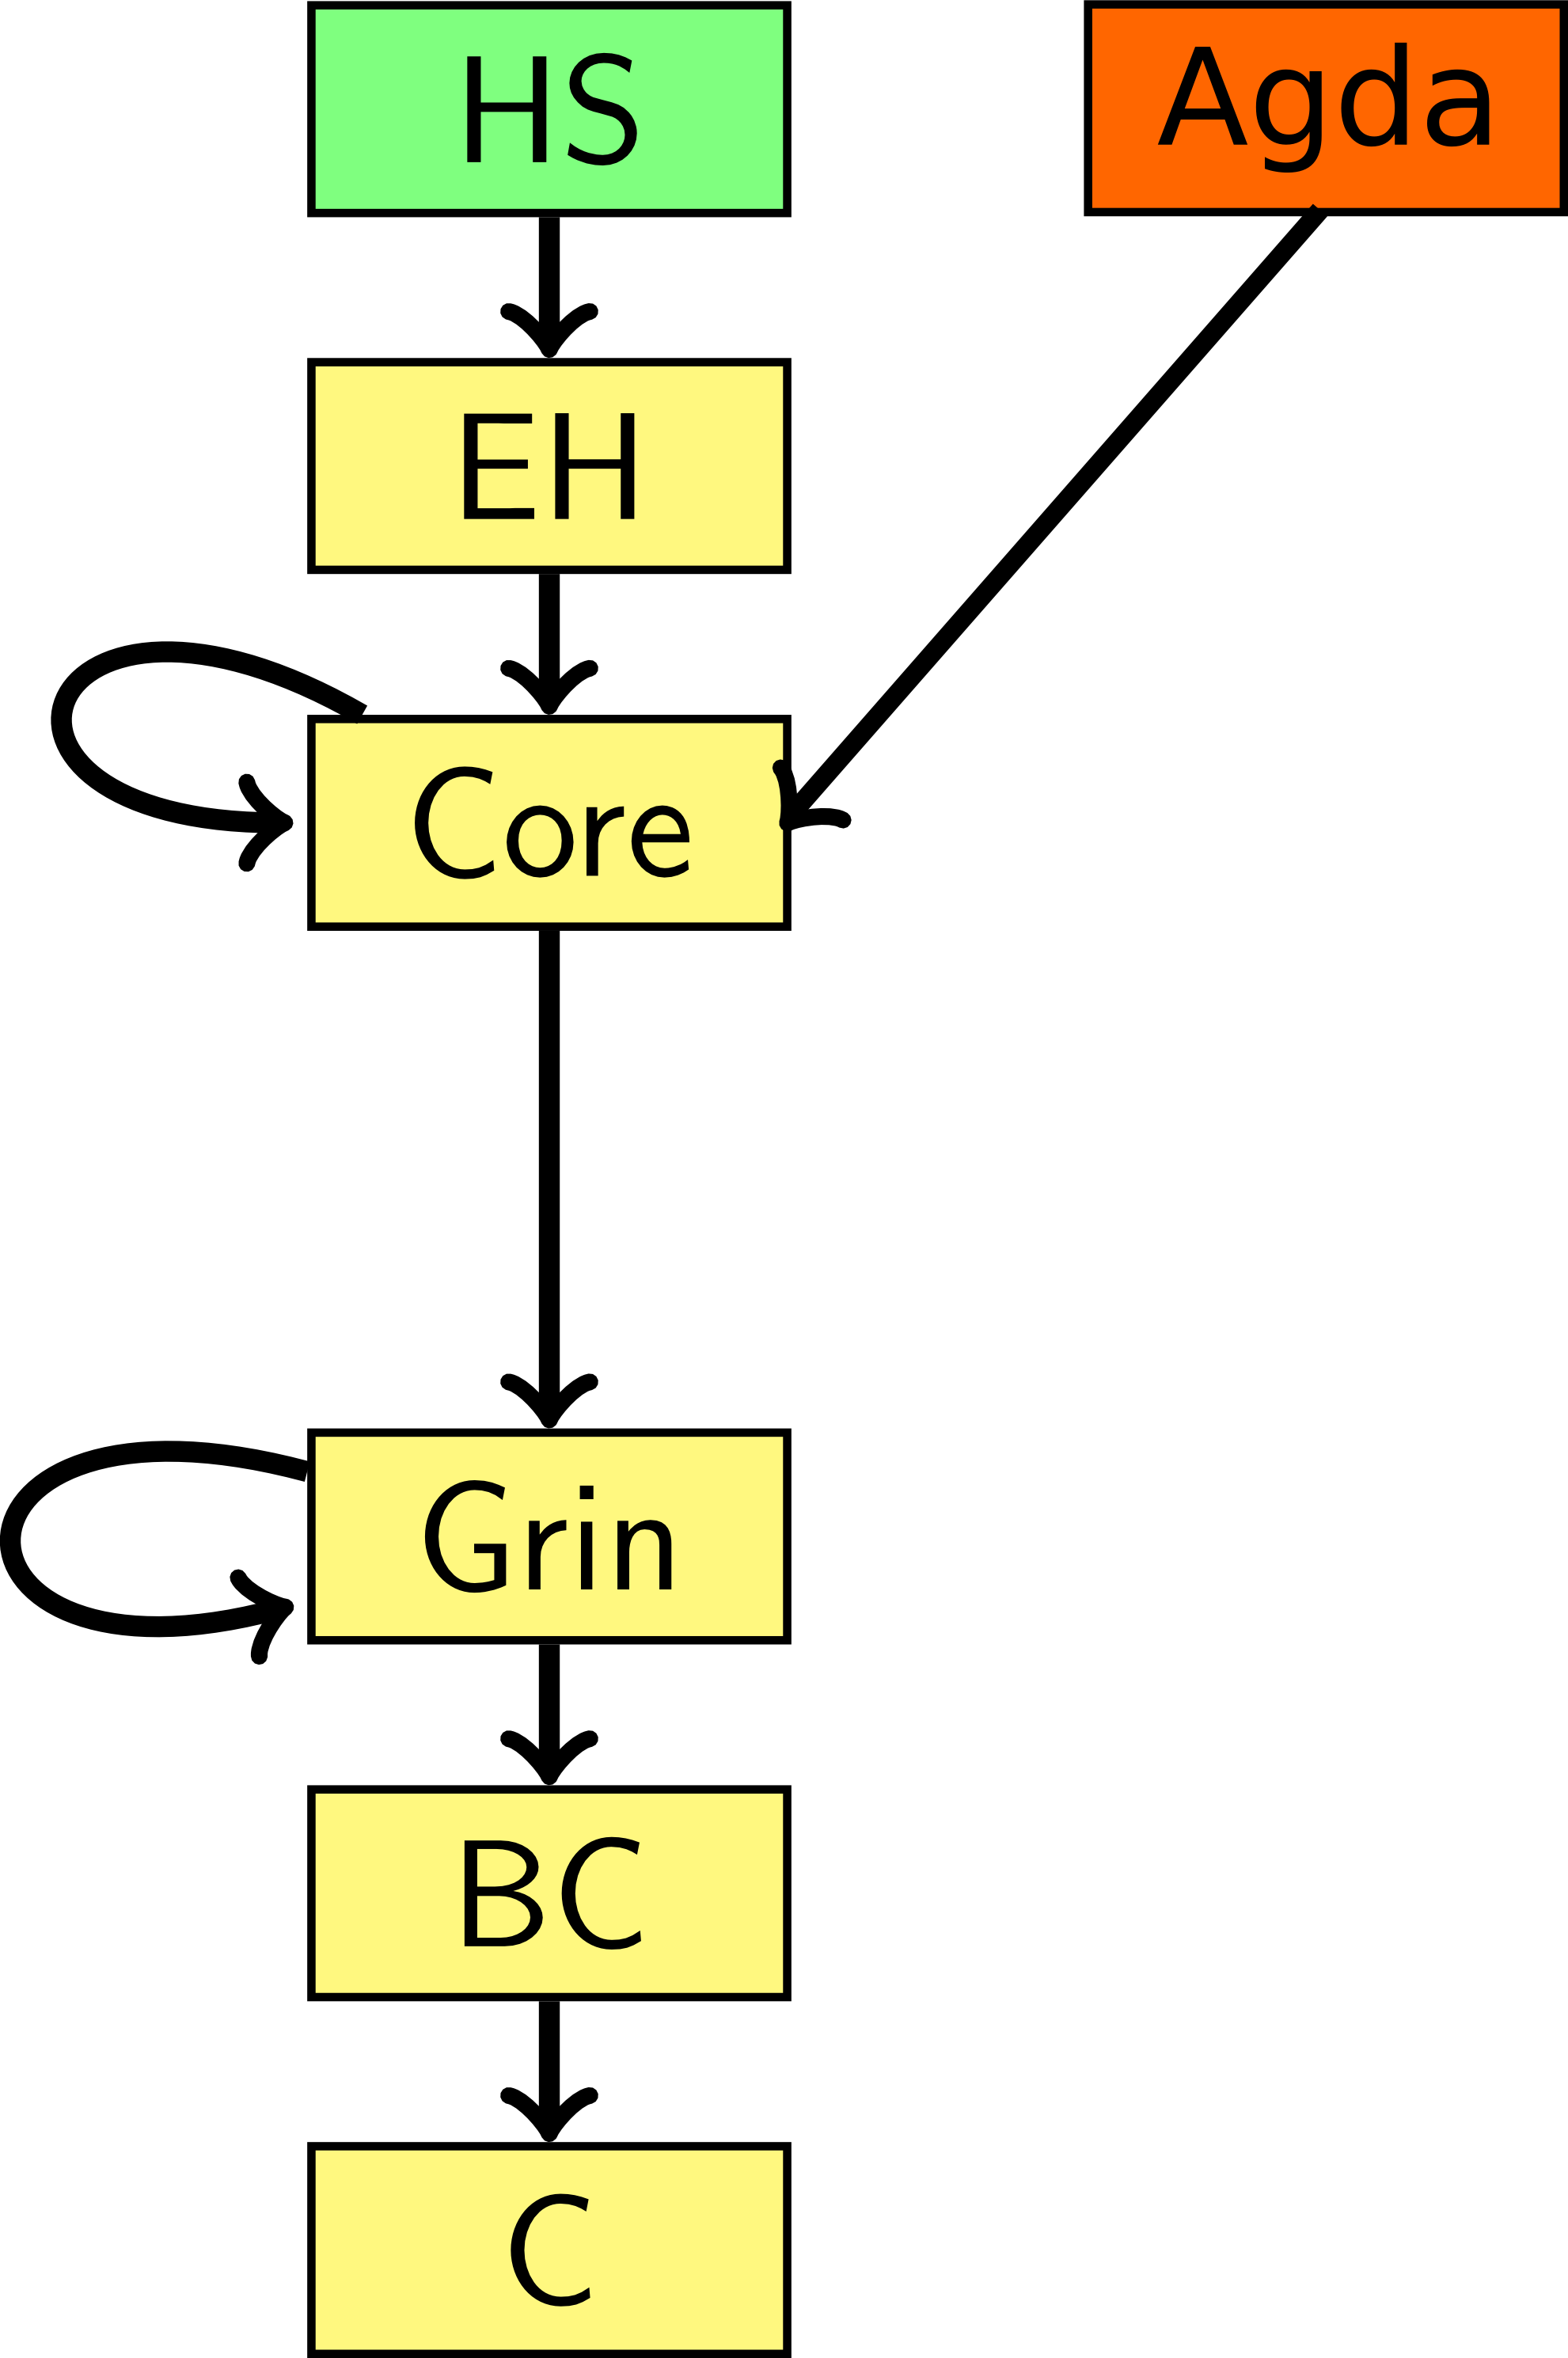
\includegraphics{uhc-arch-extr-mod.png}
\footcite{dijkstra2009architecture}
\end{frame}


\begin{frame}[fragile]{UHC Backend}
\centering
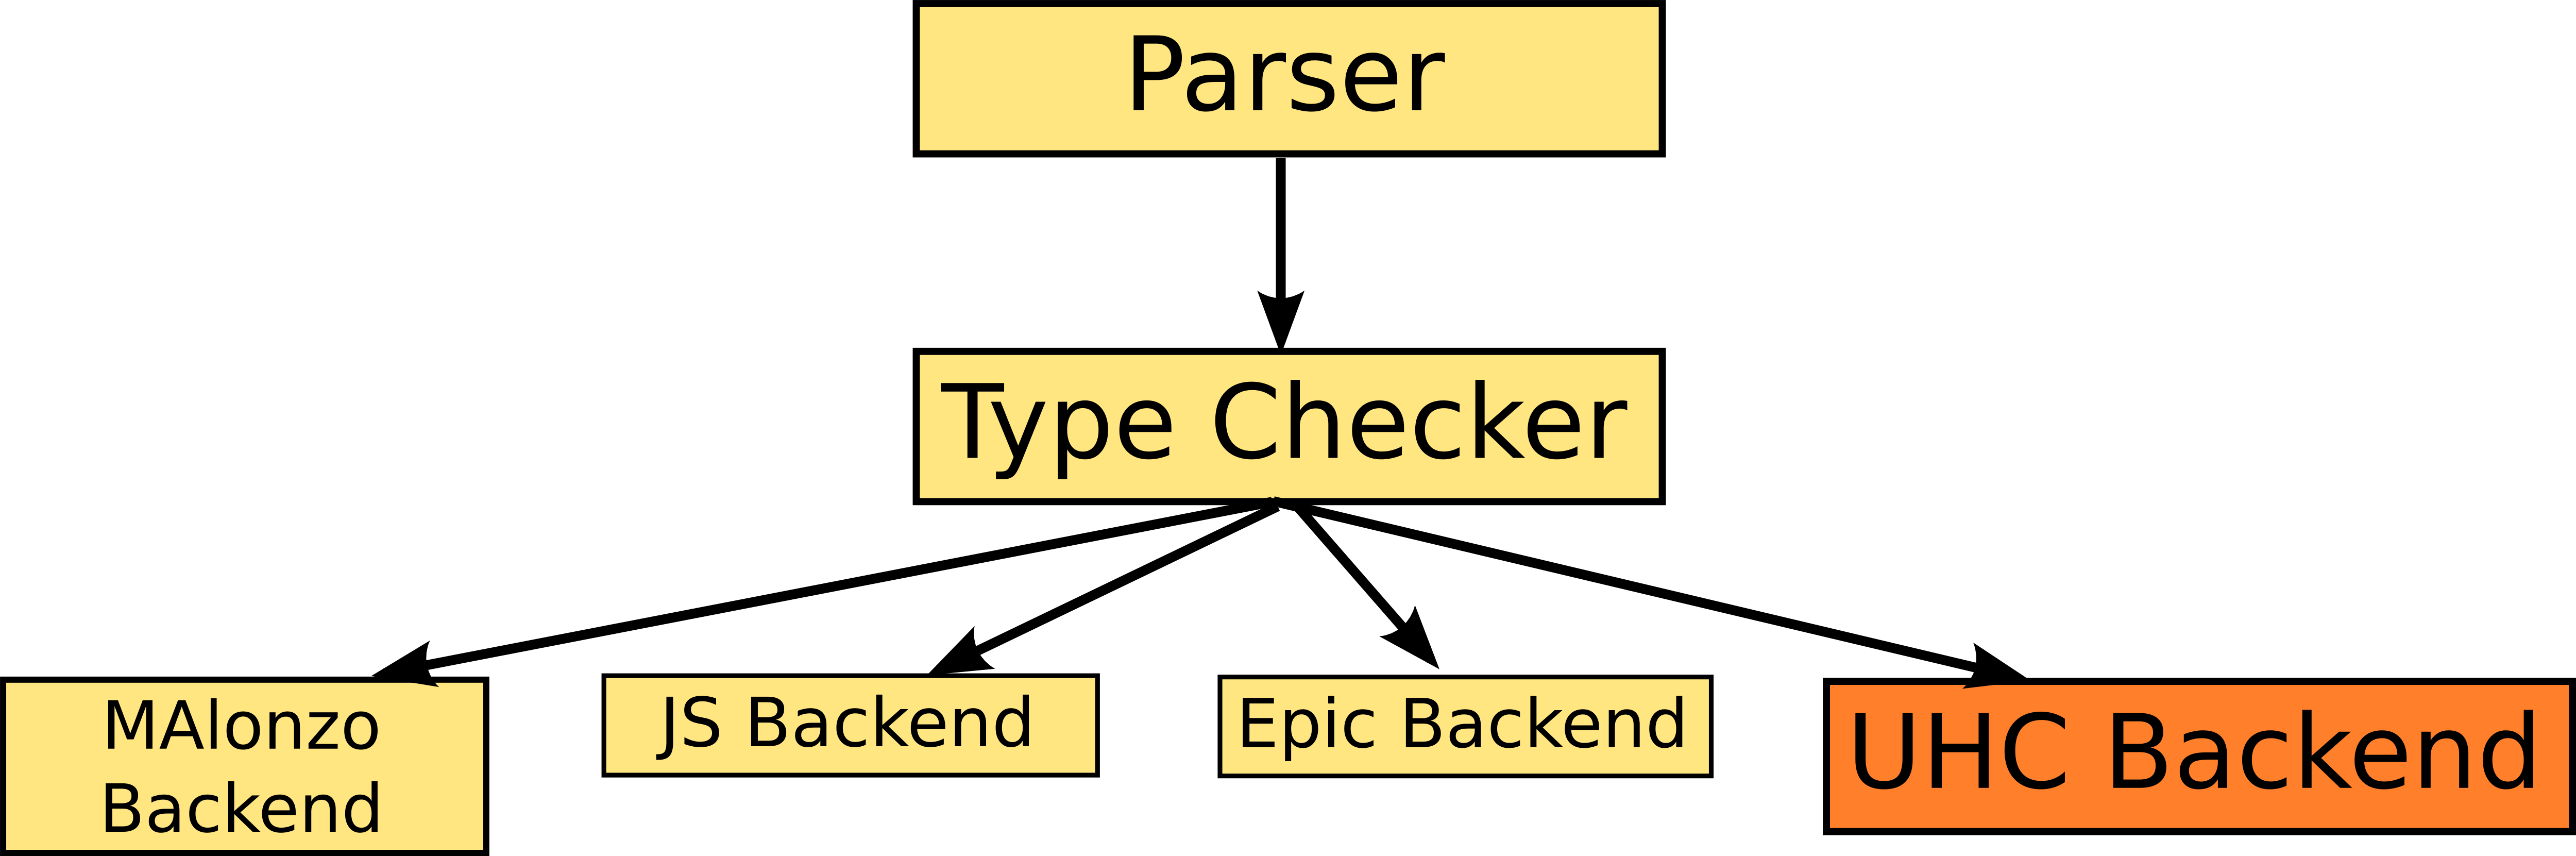
\includegraphics[width=250px]{agda-arch-with-uhc.png}
\par
\end{frame}


\begin{frame}{Epic vs UHC Core}
\begin{tabular}{c r l c r l}
\hline
\multicolumn{3}{l}{Epic Language} & \multicolumn{3}{l}{UHC Core} \\
\hline
$t$ & $::=$ & $x$               & $t$ & $::=$ & $x$ \\
& \textbar & $t$ $\vec{t}$            & & \textbar & $t$ $t$ \\
& \textbar & $\lambda x \rightarrow t$ & & \textbar & $\lambda x \rightarrow t$ \\
& \textbar & Con $i$ $\vec{t}$        & & \textbar & Con $i$ $\vec{t}$ \\
& \textbar & if $t$ then $t$ else $t$ & & & \\
& \textbar & case $t$ of $\vec{alt}$  & & \textbar & case $t$ of $\vec{alt}$ \\
& \textbar & let $x$ = $t$ in $t$     & & \textbar & let $x$ = $t$ in $t$ \\
& &                                   & & \textbar & let! $x$ = $t$ in $t$ \\
& \textbar & lazy $t$                 & & & \\
%& \textbar & $t$ $!$ $i$              & & & \\
& \textbar & $i$                      & & \textbar & $i$
%\\
%$alt$ & ::= & Con $i$ $\vec{x}$ $\rightarrow$ $t$     & $alt$ & $::=$ & Con $i$ $\vec{x}$ $\rightarrow$ $t$ \\
%& \textbar & $i$ $\rightarrow$ $t$                    & & & \\
%& \textbar & default $\rightarrow$ $t$                & & \textbar & default $\rightarrow$ $t$
\end{tabular}
\end{frame}

\begin{frame}[fragile]{UHC Backend - Challenges}
\begin{itemize}
\item Agda is a moving target
\item UHC Core was not intended as public API
\item Undocumented assumptions inside UHC
\pause
\begin{lstlisting}[language=Haskell]
case x of
  []     -> a
  (x:xs) -> b
\end{lstlisting}
is not the same as
\begin{lstlisting}[language=Haskell]
case x of
  (x:xs) -> b
  []     -> a
\end{lstlisting}
%\begin{itemize}
%    \item E.g. alt
%\end{itemize}
\end{itemize}
\end{frame}

\begin{frame}{UHC Backend - What works?}
\begin{itemize}
\item (Dependent) dataypes, functions
\item Compiling single Agda modules
\item Agda - Haskell FFI, but involves manual work
\end{itemize}
\end{frame}

\begin{frame}
Demonstration
\end{frame}

\begin{frame}{UHC Backend - Future work}
\begin{itemize}
\item Support whole Agda language
  \begin{itemize}
  \item Multiple modules
  \item Complete IO bindings
  \item Agda Standard Library
  \end{itemize}
\item Optimizations
\item Improve Agda - Haskell FFI
\item Agda support for Cabal
\item Contracts for FFI
\end{itemize}
\end{frame}

%    \input{section-dtp-agda.tex}
%    \input{section-piware-syntax.tex}
%    \input{section-piware-semantics.tex}
%    \input{section-piware-proofs.tex}
%    \input{section-final.tex}


    \begin{frame}[plain]
        \begin{center}
            \par{\Huge{Thank you!}}
            \vspace{\baselineskip}
            \par{\Huge{Questions?}}


        \end{center}
    \end{frame}

    \begin{frame}[allowframebreaks]
        \frametitle{References}
        \bibliographystyle{apalike}
        \bibliography{bib}{}
    \end{frame}
\end{document}

